\documentclass{article}
\usepackage[margin=2cm]{geometry}
\usepackage{graphicx}
\usepackage[pages=some]{background}
\usepackage{titling}
\usepackage{tabularx}
\usepackage{tikz}
\usepackage{forest}
\usepackage{amsmath}
\usepackage{amssymb}
\usepackage{multicol}
\usepackage{subcaption}
\usepackage{float}

\forestset{
  my box/.style={
    draw,
    rectangle,
    rounded corners,
    fill=gray!20,
    inner sep=6pt,
    minimum width=3cm % Adjust the width as needed
  }
}


\geometry{a4paper}

\backgroundsetup{
    scale=1,
    angle=0,
    opacity=1,
    contents={%
        
\includegraphics[width=\paperwidth,height=\paperheight]{institution_logo.jpg}
    }
}

\newcommand{\subtitle}[1]{
    \posttitle{
        \par\end{center}
        \begin{center}\large#1\end{center}
        \vskip0.5em}
}

\title{ME-463}
\author{Md. Hasibul Islam}
\subtitle{PETROLEUM ENGINEERING}

\begin{document}
\begin{titlepage}
    \centering
    
    {\Huge\bfseries\maketitle}
    \textbf{Quamrul Islam Sir} \\
    \vspace{2cm}
    
\includegraphics[width=8cm]{institution_logo.jpg}
    \vfill
    \vspace*{2cm}
\end{titlepage}

\tableofcontents
\pagebreak
\section{Lecture 01: Introduction} 
\subsection*{\hfill Date: 03/06/2023}

\subsection*{Booklist}

\textbf{Introduction of Petroleum Geology \& Drilling}

\hfill Published by BUET

\subsection*{Basics}

\begin{tabular}{@{}p{1\textwidth}@{}}
Latin: \textbf{Petra} → Rock or Stone \\
Latin: \textbf{Oleum} → Oil \\
So, Petroleum basically means "Rock Oil"\\
\\

Petroleum occurs widely in the earth as gas, liquid, semi-solid or solid, or in more than one state in a single place.
\end{tabular}
\\

\subsection*{Definition}
Chemically, any petroleum is an extremely complex mixture of hydrocarbon (hydrogen and carbon) compounds with minor amounts of nitrogen, oxygen, and sulfur as impurities. The weight percentage of petroleum is as follows:
\\
\begin{center}
\begin{tabularx}{\textwidth}{X X}
  \hline
  \textbf{Elements} & \textbf{Amount} \\
  \hline
  Carbon & 85\%-90\% \\
  Hydrogen & 10\%-15\% \\
  Sulfur & 0.2\%-5\% \\
  $N_{2}$ & 0.1\%-2\% \\
  $O_{2}$ & 0.6\%-2\% \\
  \hline
\end{tabularx}
\end{center}

\vspace{1cm}
% trees 
\begin{center}
  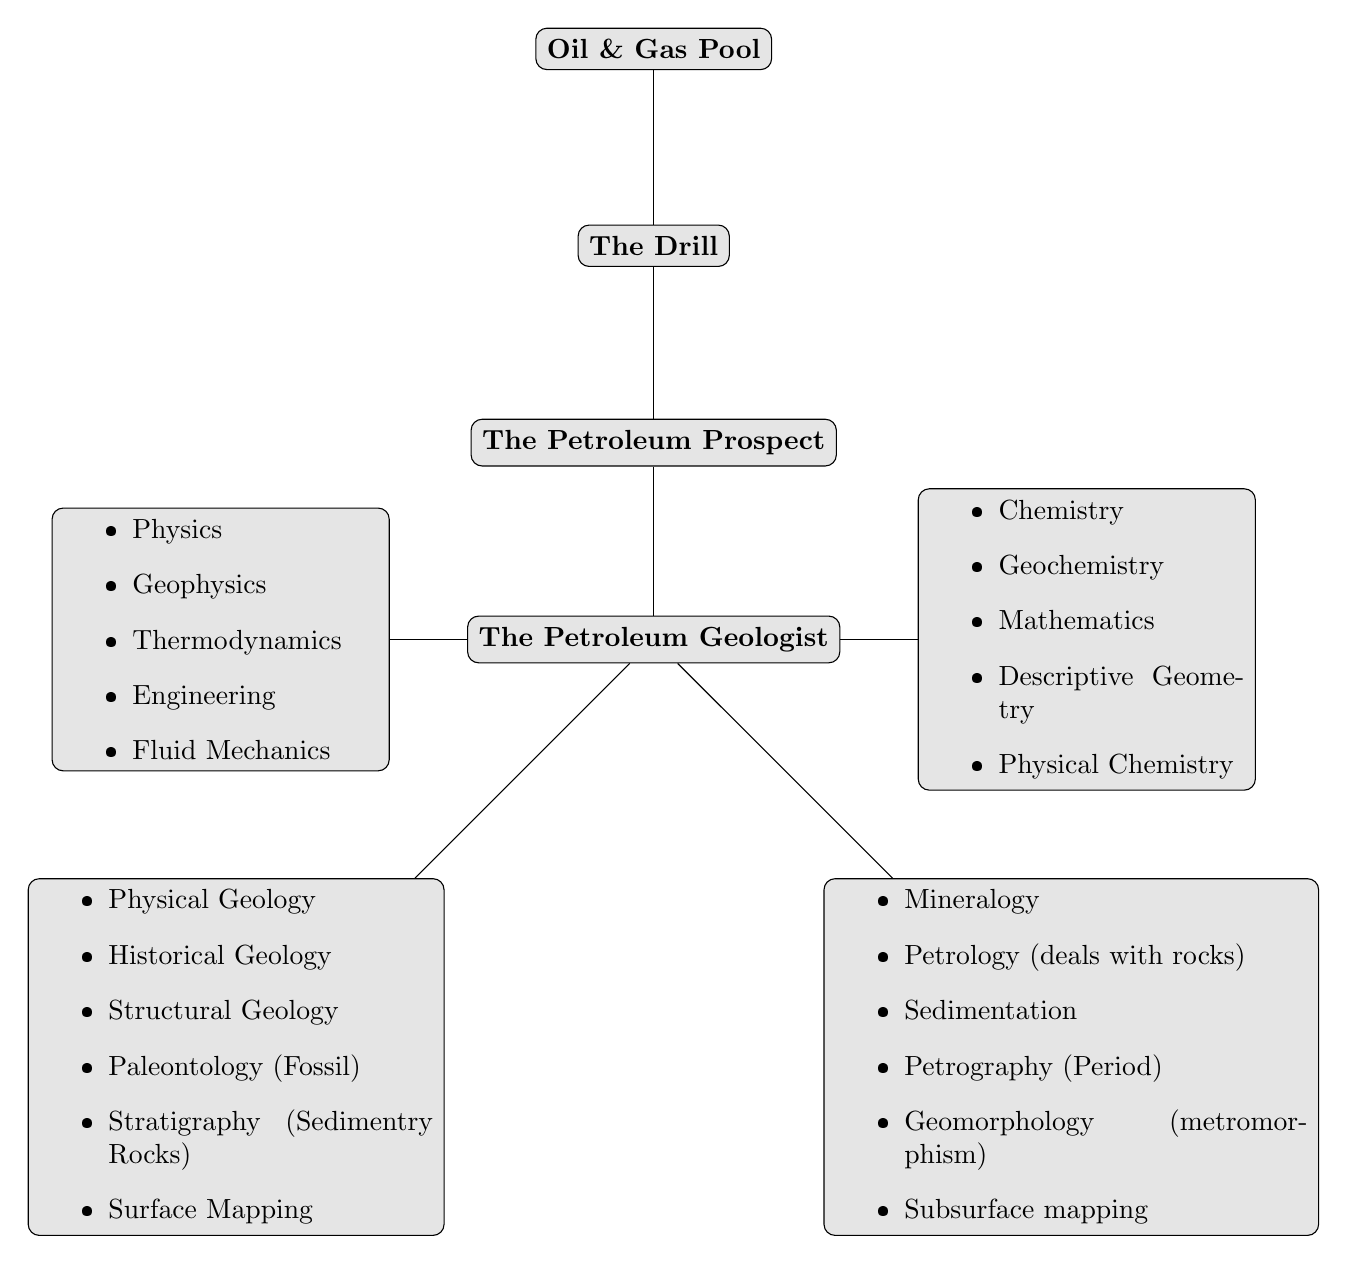
\begin{tikzpicture}[level distance=2cm,
    level 1/.style={sibling distance=2cm},
    level 2/.style={sibling distance=2cm},
    level 4/.style={sibling distance=4cm}, % Adjust the sibling distance for level 4
    box/.style={draw, rectangle, rounded corners, fill=gray!20, inner sep=4pt}]
    \node[box] {\textbf{Oil \& Gas Pool}}
      child[grow=down, level distance=2.5cm] {node[box] {\textbf{The Drill}} % Changed level one node label
        child[grow=down, level distance=2.5cm] {node[box] {\textbf{The Petroleum Prospect}}
          child[grow=down, level distance=2.5cm] {node[box] {\textbf{The Petroleum Geologist}}
            child[grow=left, level distance=5.5cm] {node[box] {
              \begin{minipage}{4cm}
                \begin{itemize}
                  \item Physics
                  \item Geophysics
                  \item Thermodynamics
                  \item Engineering
                  \item Fluid Mechanics
                \end{itemize}
              \end{minipage}
            }}
            child[grow=south west, level distance=7.5cm] {node[box] {
              \begin{minipage}{5cm}
                \begin{itemize}
                  \item Physical Geology
                  \item Historical Geology
                  \item Structural Geology
                  \item Paleontology (Fossil)
                  \item Stratigraphy (Sedimentry Rocks)
                  \item Surface Mapping
                \end{itemize}
              \end{minipage}            
            }}
            child[grow=south east, level distance=7.5cm] {node[box] {
              \begin{minipage}{6cm}
                \begin{itemize}
                  \item Mineralogy
                  \item Petrology (deals with rocks)
                  \item Sedimentation
                  \item Petrography (Period)
                  \item Geomorphology (metromorphism)
                  \item Subsurface mapping
                \end{itemize}
              \end{minipage}            
            }}
            child[grow=right, level distance=5.5cm] {node[box] {
              \begin{minipage}{4cm}
                \begin{itemize}
                  \item Chemistry
                  \item Geochemistry
                  \item Mathematics
                  \item Descriptive Geometry
                  \item Physical Chemistry
                \end{itemize}
              \end{minipage}            
            }}
          }
        }
      };
  \end{tikzpicture}
\end{center}

\vspace{2cm}
\subsection*{Petroleum Geology}
Geology is the sciecne that deals with the history and structure of the earth and its life forms. It is used to credit where oil accumulation might occur. Geology is based on observation and the knowledge derived from mant others sources.
\\

% horizontal tree

\begin{center}
  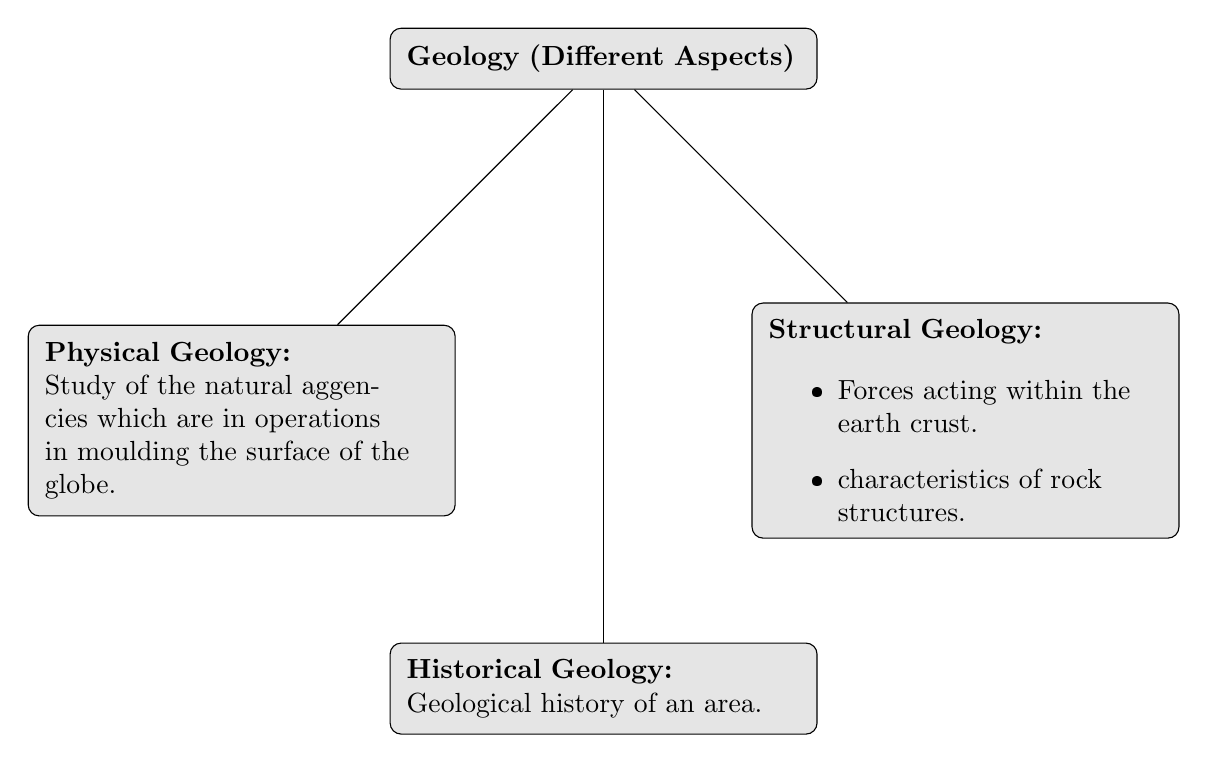
\begin{tikzpicture}[level distance=5cm,
    level 1/.style={sibling distance=5cm},
    level 2/.style={sibling distance=5cm},
    level 3/.style={sibling distance=5cm},
    box/.style={draw, rectangle, rounded corners, fill=gray!20, inner sep=6pt, text width=5cm}]
    \node[box] {\textbf{Geology (Different Aspects)}}
           child[grow=south west, level distance=6.5cm] {node[box] {
        \textbf{Physical  Geology:}\\ 
        Study of the natural aggencies which are in operations in moulding the surface of the globe.
      }}
      child[grow=down, level distance=8cm] {node[box] {
        \textbf{Historical Geology:} \\
        Geological history of an area.
      }}
      child[grow=south east, level distance=6.5cm] {node[box] {
        \textbf{Structural Geology:} \\
        \begin{itemize}
                  \item Forces acting within the earth crust.
                  \item characteristics of rock structures.
                  \end{itemize}
}};
  \end{tikzpicture}
\end{center}
\vspace{2cm}
\subsection*{Petroleum Geologiest (activities)}
\begin{center}
\begin{itemize}
    \item Observes the rock and rock formations.
     \item Reconstructs the geological history of an area 
     \item Determines whether the formations contains petroleum in the reservoirs. 
\end{itemize}
\end{center}



\newpage

\section{Lecture 2: Petroleum Classification}
\hfill Date: 17/06/2023

\paragraph*{} A petroleum deposit must be commercially valuable. it depends on some factors: 
\begin{enumerate}
  \item Amount recoverable 
  \item Expected production rate 
  \item Cost of drilling and producing well
\end{enumerate}

$\checkmark$ if there is fire in well, then another well should be dug nearly to reach there. 

\subsection*{Petroleum Reservoir characteristics}
A good reservoir must have: 
\begin{itemize}
  \item Right shape or configuration to hold the oil and some kind of seal or trap to keep it from escaping
  \item it must be large enough usually 10 ft thick or more. 
  \item About 10\% porosity or pore space in needed.
  \item It must be permeable, that is, pores must be connected so that, oil, gas and water can flow through it from one pore to another. 
\end{itemize}

$\checkmark$ Sandstone $\rightarrow$ Porous

\subsection*{Petroleum Classification}
The petroleum and petroleum like substance may be classified as follows: 
\begin{enumerate}
  \item \textbf{Petroleum} : An almost infinitely complex mixure of saturated hydrocarbon with relatively small amounts of $S,N_2, O_2$ and many other lesser constituents in combination. Petroleum occurs in solid, liquid and gaseous forms as follows : 
  \begin{enumerate}
    \item Asphalt or tar, paraffin waxes, brittle bitumen etc.
    \item Crude oils (liquids)
    \item Natural Gas 
  \end{enumerate} 
  \item \textbf{Tar Sands}: Semi-solid petroleum bearing sands 
  \item \textbf{Oild Shales}: These are fine grained sediments sometimes known as kerogen shales. 
  \item Torbanites, boghead and cannel coal etc all are rich in bitumen 
\end{enumerate}

$\checkmark$ Fishing $\rightarrow$ If drill bit is broken inside well \\
$\checkmark$ Catwalk $\rightarrow$ pipe movement through crane 

\subsection*{Age of the earth (Structure of the earth)}
it is very difficult to ascertain the actual and exact of the earth. 
\begin{itemize}
  \item Darwin fixed the age of the earth at 57 billion years on the basis of the concept of separation of the moon from the body of the earth.
  \item Through the study of the history of cooling of the earth, calvin estimated that our planet should be as old as 20 to 40 million years 
  \item Study of radioactive naterials in meteorites indicate that the members of the solar system must be as old as about 4500 million years 
  \item Modern theory is that the earth is thought to have formed about 4.6 billion years ago out of a cosmic dust. As the planet was pulled together due to its own gravity, the heat of compression and of it's radioactive elements caused it to become molten. The heaviest components form the core. Lighter minerals form the thick mantle. The lighter elements form the thin rocking crust. 
\end{itemize}


\section{Lecture 3: Internal Structure of the earth crust}
\hfill Date: 08/07/2023 

Internal structure of the earth consists of the followings:
\begin{enumerate}
  \item Earth crust 
  \item Mantle 
  \item Core 
\end{enumerate}

\subsection*{Earth Crust (Lithosphere)}
Outer envelope of shell of the earth is known as earth crust. This crust consists of solid rocks. The thickness of earth crust ranges from 5 to 70 km.

Two part of earth's crust:\\
i) Outer crust \\
ii) Lower crust 

\vspace*{0.5cm}
The earth's outer crust mainly consists of sedimentary rocks. \\
Outer crust:\\
i) Continental crust (30 km thick, average specific gravity 2.8, high over 0.2 to 0.3 km above sea)\\
ii) Oceanic crust (5km thick, average specific gravity 2.9, 4 to 5 km sea level)

\begin{figure}[H]
  \begin{center}
    \includegraphics*[width=0.6\linewidth]{img/cross_section_earth.jpg}
    \caption{Cross section of Earth}
  \end{center}
\end{figure}
\begin{figure}[h]
  \begin{center}
    \includegraphics*[width=0.6\linewidth]{img/Crust.png}
    \caption{Outer crust \& inner crust} 
  \end{center}
\end{figure}

\vspace*{0.5cm}
The lower part of earth crust has two envelopes. \\
Lower crust: \\
i) Granite Layer \\
ii) Basalt Layer \\

\vspace*{0.5cm}
The average thickness of each of this layer ranges from 15 to 20 km. 


\subsection*{Tectonic Plates and Plate Boundaries}
Lithosphere consists of spherical caps or plates. These plates are in relative motion to each other on the non-rigid asthenosphere. \\
There may be a - 
\begin{itemize}
  \item Collision
  \item Pulling away 
  \item Slide Past one another 
\end{itemize}

The theory that explains this processes is called plate tectonic theory.

\vspace*{1cm}

Plates may be - 
\begin{itemize}
  \item Continental (Eurasian Plate) \\ - Thick and relatively light.
  \item Oceanic (Pacific Plate) \\ - Thin and made up of wavy igneous rocks.
\end{itemize}

Mountain ranges, ocean basins, major features of earth etc are found due to the movement of plate boundaries. 

\begin{figure}[H]
  \begin{center}
    \includegraphics*[width=0.7\linewidth]{img/lithospehere.png}
    \caption{Plastic Higher Temperature Layer\\ (Asthenosphere 100 to 200 km)}
    Lower part of earth's crust 
  \end{center}
\end{figure}


\subsection*{Classification of Plate Boundaries} 
Three types of plate boundaries exist:
\begin{enumerate}
  \item Divergent Boundaries 
  \item Convergent Boundaries 
  \item Transcurrent Boundaries 
\end{enumerate}
\hrulefill

\section{Lecture 4: Internal Structure of the earth}
\hfill Date: 08/07/2023 

\begin{multicols*}{2}
  \subsection*{ii) Mantle}
  \subsubsection*{characteristics:}
  \begin{itemize}
    \item Next to earth's crust 
    \item Rich in Al, Si, Mg 
    \item 2900 km thick 
  \end{itemize}

  It has three sections:
  \begin{enumerate}
    \item Upper mantle: 40 to 200 km below the earth's surface 
    \item Middle mantle: At a depth of 200 to 1000 km 
    \item Lower mantle: 1000 to 2900 km below the surface of the earth 
  \end{enumerate}
  Maximum temperature of these section in 2200°C. 

  \subsection*{iii) Core}
  \subsubsection*{charateristics:}
  \begin{itemize}
    \item Next to mantle 
    \item About 3400 km radius 
    \item two parts: Outer core \& Inner core 
  \end{itemize}

  \subsubsection*{Outer Core:}
  \begin{itemize}
    \item Temperature 2200°C to 5000°C 
    \item Consists of hot molten nickel, cast iron etc. 
  \end{itemize}

  \subsubsection*{Inner Core:}
  \begin{itemize}
    \item The temperature is 5000°C 
    \item Consists of solid balls of iron and nickel.
    \item  The atoms of the metal are pressed together so tightly by gravity that melting is impossible.  
  \end{itemize}

  \subsection*{Tectonic Plates and Plate Boundaries}
  \subsubsection*{(a) Divergent Boundaries:}
  It is a tensile regime, as the two plates of the continent diverges or separates, magma rises from mantle after solidification forms mid-ocean ridge. 

  Example: About 200 million years ago, the atlantic ocean was born in this process. 

  % 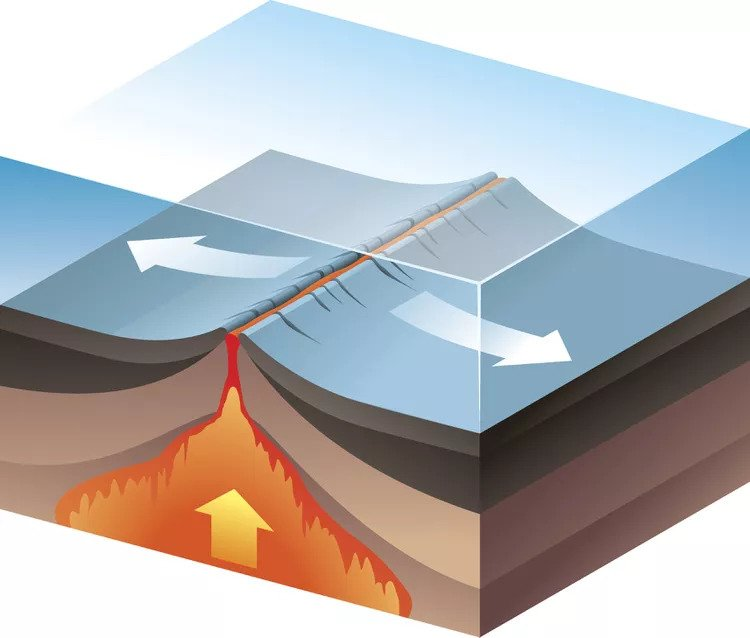
\includegraphics[width=\columnwidth]{img/divergent_boun.jpg}


  \subsubsection*{(b) Convergent Boundaries:}
  It is a compressional regime and several things can happen. 
  \begin{itemize}
    \item Ocean-ocean convergent boundaries 
    \item Ocean-continent convergent boundaries 
    \item Continental-continental convergent boundaries 
  \end{itemize}

  \subsubsection*{Ocean-Ocean convergent boundaries:}
  One plate slips beneath the edge of the other. The lower plate is melted as it moves into the hot mantle. The melting minerals rises through the crust forming granite and other igneous rocks.

  Example: South sandwich trench of atlantic ocean formed in this way. 

  \subsubsection*{Ocean-Continent Convergent Boundaries:}
  Thinner and heavier oceanic plate plunges beneath continental crust, forming a deep sea trench. Magma rises from descending pipe.

  Example: Mount saint helens volcanos formed in this way.

  \subsubsection*{Continent-continent Convergent Boundaries:}
  The collision buckles and folds the rocks.
\end{multicols*}

\begin{figure}[H]
  \centering
  
  \begin{subfigure}[b]{0.45\textwidth}
    \centering
    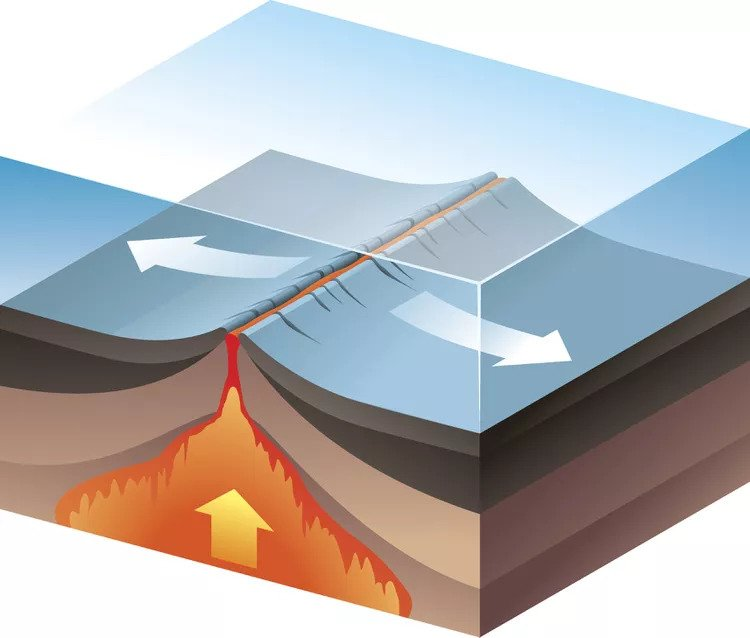
\includegraphics[width=\textwidth]{img/divergent_boun.jpg}
    \caption{Divergent Boundaries}
    \label{fig:subfig1}
  \end{subfigure}
  \hfill
  \begin{subfigure}[b]{0.45\textwidth}
    \centering
    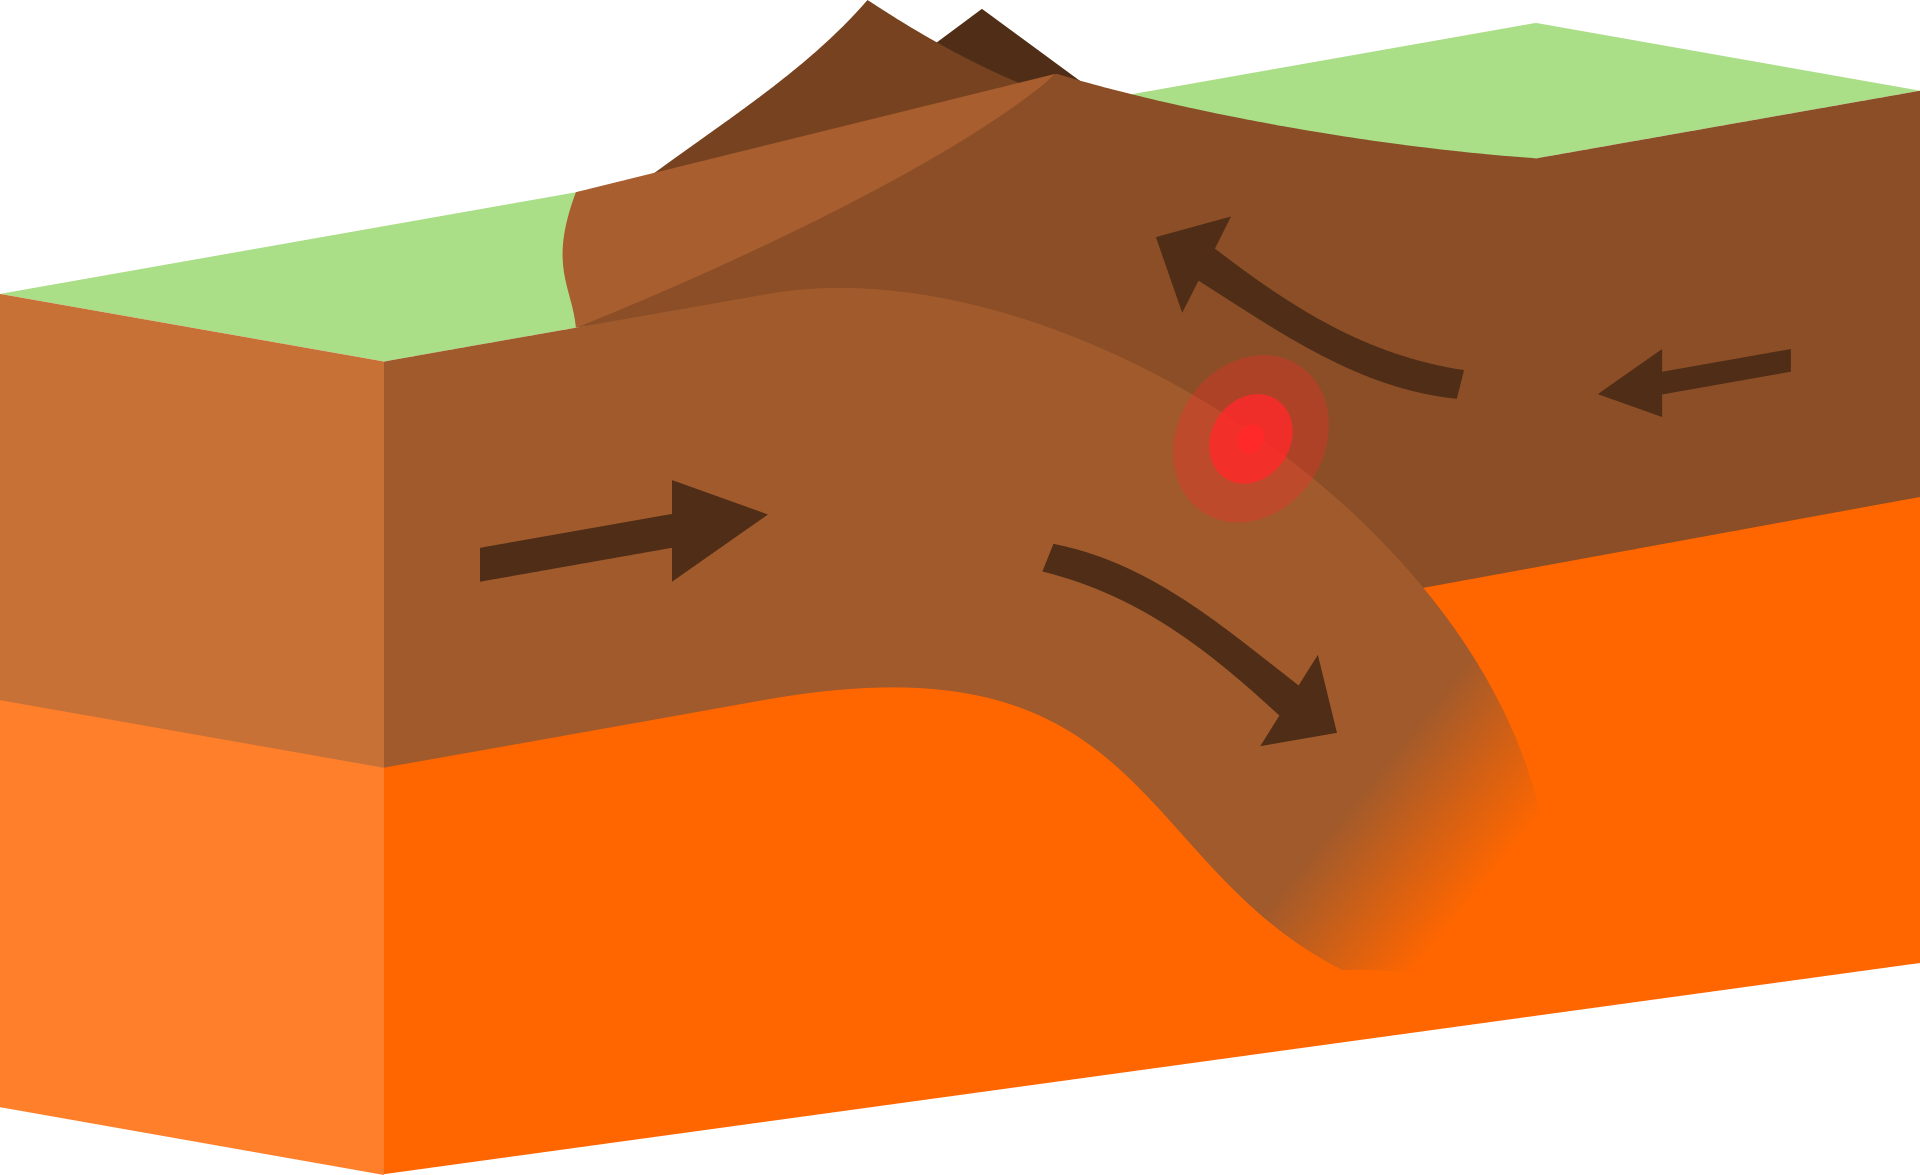
\includegraphics[width=\textwidth]{img/convergent_boun.png}
    \caption{Convergent Boundaries}
    \label{fig:subfig2}
  \end{subfigure}
  
  \caption{Tectonic Plates and plate boundaries}
  \label{fig:mainfig}
\end{figure}
   
\end{document}
